\up
%\begin{compactenum}[a)]
\emph{Scientific objectives:} The objective of this work is to %calculate the properties of clay platelets immersed in a polymer matrix (a nanocomposite system) and to 
investigate the complex interaction between bio-molecules and clay-mineral systems relevant to origins of life and applications to drug delivery. 
This work is supported by UK EPSRC RealityGrid Platform Grant (EP/C536452/1), 
an EPSRC PhD studentship and the UK Technology Strategy Board's NIMES (Q2506L) project.
Hitherto, research into the origins of life has rarely used simulation techniques to understand the possible chemical pathways to the formation of early bio-molecules. The main purpose of this research is to use computer simulation to provide insight into the structure, conformation and stability of nucleic acids while interacting with a clay surface, both intercalated between the layered minerals and adsorbed onto the edge of the layered mineral. Such insight is difficult to obtain experimentally due to the disordered nature of these systems. From the increased computational power of the TeraGrid, it is possible to effectively model realistic sized fully atomistic models which can simulate an aqueous clay surface and incorporate large bio-molecules, such as ribozymes, whilst removing finite size effects \cite{JPCC_2007}. It is also now possible to access timescales in the range of hundreds of nanoseconds where previously only tens of nanoseconds were accessible, in conceivable real-time. These increased timescales are particularly relevant for large complex nucleic acid (RNA \& DNA) molecules in which folding of the molecule into functional tertiary structures happens over long timescales. 

In nature, clay materials are composed of platelets approximately 1
micrometre wide and, in  bio- and non-bio composites, these platelets are dispersed in a matrix of 
polymer chains.  In conventional molecular dynamics simulations of nanocomposites, a small simulation cell is replicated to represent an infinite clay platelet. This is an approximation that we have started to remove in our studies and will now apply to biomolecular -clay systems, by creating very large clay systems which can accommodate large complex bio-polymers, and also by examining isolated clay platelets, with edges, of realistic size. 

In an extension to our previous bio-clay nanocomposite work, we plan to explore the mechanism by which RNA adsorbs on external aqueous montmorillonite mineral surfaces, using molecular dynamics (MD) techniques, to look at the interaction of RNA of differing base sequences with the mineral surface in the presence of differing charge balancing cations. This will give a molecular level understanding of the mechanism by which RNA adsorbs/interacts with the montmorillonite surface to support experimental findings of these systems \cite{Franchi, Huang}. Other work will look at the relative structural stability of free and layered Mg-Al double hydroxide intercalated nucleic acids, at temperatures and pressures relevant to origins of life studies, see Figure \ref{F:pics} (contained within this document). For both clay systems we will firstly study the interaction of RNA intercalated within the clay framework (i.e. the basal surface).  From these simulations it will be possible to calculate the mean-squared displacement and the radius of gyration of the bio-molecule as well as finding the dominant modes of motion through principal component analysis. Radial distribution functions, atomic density profiles and time-averaged visualizations of the systems will provide the structure and conformation of the whole system.
 
\begin{figure} 
        \begin{center}
           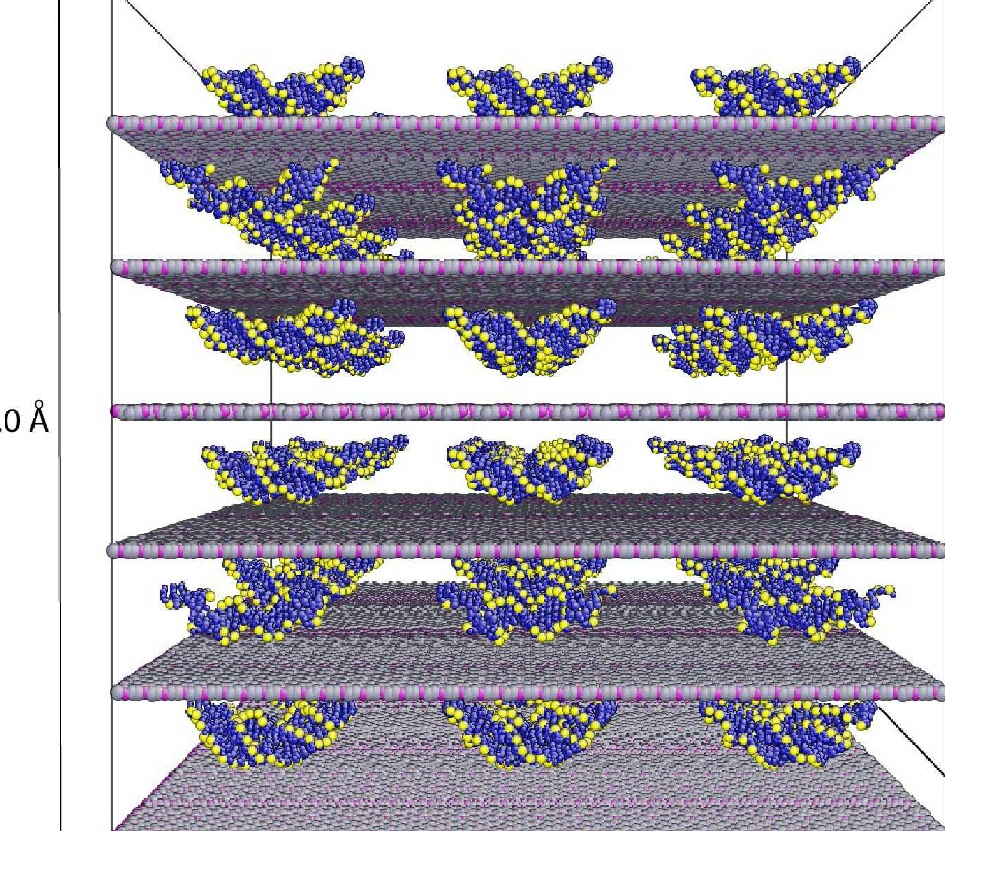
\includegraphics[scale=0.3]{subproject1-bioclays/pic1}
           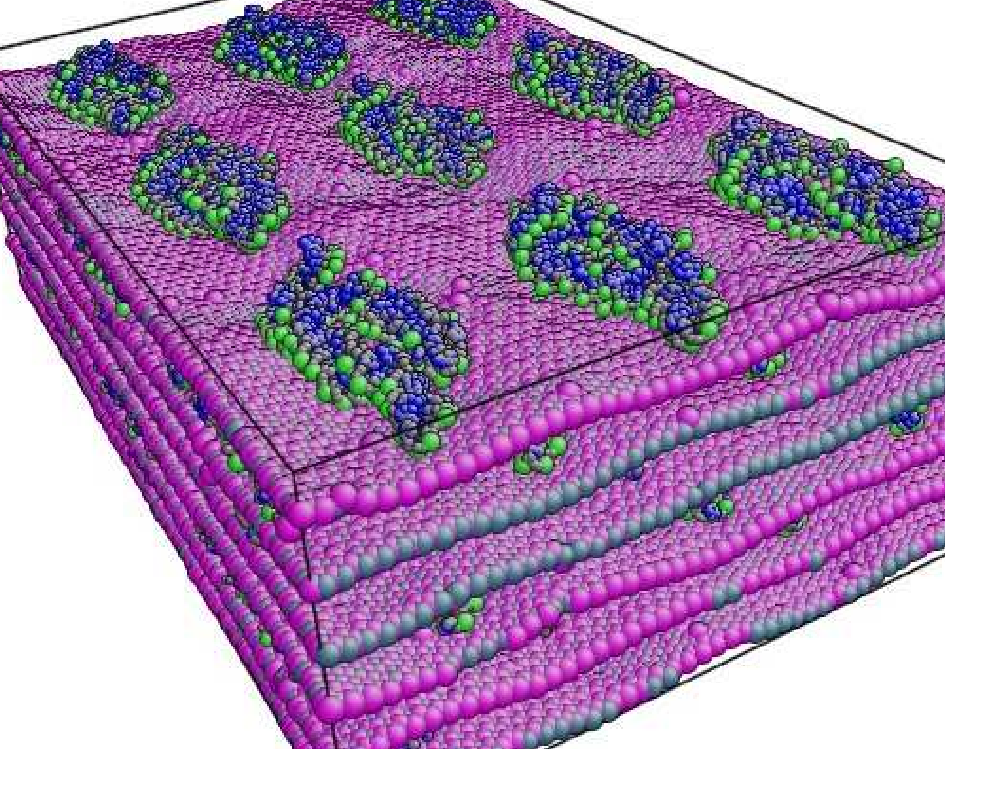
\includegraphics[scale=0.3]{subproject1-bioclays/pic2}
           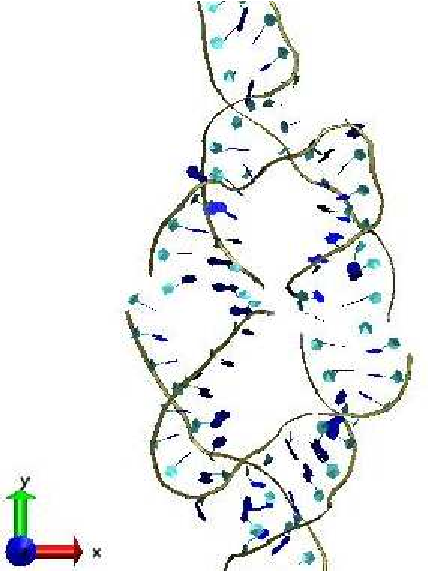
\includegraphics[scale=0.3]{subproject1-bioclays/pic3}
        \end{center}
%\caption{Visualizations of a hammerhead ribozyme intercalated into an LDH clay mineral consisting of 1,181,736 atoms.}
        \caption{\small Initial stucture of the hammerhead ribozyme intercalated into an LDH clay mineral at the start of simulation (a) consisting of 1,181,736 atoms.  Magnesium, aluminium, chlorine, phosphorus, carbon and nitrogen atoms are represented as light grey, pink, green, yellow, dark grey and blue spheres respectively. (b) Final stucture of the large LDH-ribozyme model after the 3.5ns production phase of simulation.  Magnesium, aluminium, chlorine, phosphorus, carbon and nitrogen atoms are represented as light grey, pink, green, yellow, dark grey and blue spheres respectively.  All nucleotide motion within the LDH sheets is significantly restricted compared to that in bulk water. In addition, visualisation reveals properties such as thermal undulations in the LDH sheet, as well as corrugation of the layers around the nucleotides. (c) Visualisation of the ribozyme molecule after 3.5ns of simulation, using ribbon notation.}
\label{F:pics}
\up
\end{figure}

%To Each model will include several dispersed ($Na^{+}$ montmorillonite) platelets immersed in either i) a matrix of poly(ethylene glycol) polymer  and ii) large biomolecules such as RNA in aqueous solution. 
%From these simulations will we perform several non-equilbrium molecular dynamics simulations (NEMD), from which we will  calculate material properties, including the bending modulus, Young's
%modulus and Poisson's ratio. %We will also be able to study the interactions between seperate platelets, which may determine the rheology of clay nanocomposites .  It is the increased mechanical and
%thermochemical stability of clay-polymer nanocomposites that has
%received much attention recently in a variety of industries
%\cite{Pinnavaia_book}; 
%our objective is to gain a greater understanding of this enhancement through these
%
%simulations. 
Secondly, we will consider the adsorption of smaller RNA molecules on the edge of clay platelets. 
This will give us insight into the mechanism of
intercalation in these compounds, required for understanding their formation. This is important not just for origins of life studies, but also in the processing conditions for drug delivery applications. For example, we will be able to see changes in the clay sheet conformation that occur with initial intercalation of the bulky biopolymers, such as the layers moving apart from each other, and whether the flexibility of the clay sheet plays a significant role. 

To approach a realistic sized platelet for long simulation times, we require system sizes 
of order 1 - 20 million atoms. The largest system will include several isolated platelets of 
realistic size with biopolymers interacting with the clay sheet edges. This size of simulation 
is now firmly within the mesoscopic regime but simulated in full atomistic detail. We shall 
include non equilibrium simulations to simulate the conditions required for the bulky biopolymers 
to intercalate between the clay sheets on a timescale we can observe with atomistic molecular 
dynamics. These non-equilibrium conditions include compressive stress and shear, which effectively 
force the biopolymers into the clay interlayer region.
%To approach a realistic sized platelet for the long simulation times, we require system sizes of order 1 - 20 million atoms. The largest system will include several isolated platelets of realistic size with biopolymers interacting with the clay sheet edges. This size of simulation is firmly within the `mesoscopic' regime but simulated in full atomistic detail. We shall include non-equilibrium simulations to understand the response of these systems to compressive / extensive stress and under shear. 

%\textbf{Principal scientific objectives} We aim to calculate the
%structural, dynamical and materials properties of a clay platelet
%($Na^{+}$ montmorillonite) immersed in a matrix of poly(ethylene glycol)
%directly from large scale molecular dynamics simulations.
% Additionally  The mechanism of intercalation in clay-polymer
%nanocomposites is unknown, and this will provide valuable
%insight.

%\item\emph{Previous Work on the TeraGrid}
%Publications and progress made in the past year on TG resources.
%In our previous simulations we utilized periodic
%boundaries on the clay sheets, allowing a simulation cell to represent
%an infinite clay platelet \cite{JPCC_2007,Thyveetil,Thyveetil_JACS, Soft_Matter1}.  
%These large-scale, fully atomistic
%simulations, 
%approached the size of a physically realistic platelet.
%From
%this, we were able to calculate mesoscopic and macroscopic properties
%directly from  molecular dynamics simulations in the absence of
%finite-size effects of both clay nanocomposites\cite{JPCC_2007,Thyveetil, Soft_Matter1} and bio-%composites~\cite{Thyveetil_JACS}.

%Using the last LRAC allocation we extended these simulations to calculate 
%the mechanical response of poly(ethylene oxide) polymer-clay nanocomposites, 
%separating the response into contributions from the polymer and clay 
%mineral layer~\cite{Soft_Matter1}. This separation technique allowed us 
%to determine how the clay-polymer elastic properties change with distance 
%from the clay surface. This is the first time the effect of mineral layers 
%on the elastic modulus of polymeric materials in the vicinity of a mineral 
%surface has been calculated. This result is a vital first step to 
%understanding the enhancement mechanism of nanocomposites and the role of 
%the very large surface area of the clay mineral layer on the surrounding medium. To simulate a 
%realistically sized clay platelet required very large scale simulations, made possible using the resources available via 
%the LRAC allocation. 

%We have also examined the mechanisms by which clay mineral layers buckle in clay-polymer nanocomposites under compressive stress. We find that a clay sheet remains stable in a flat state until a critical compressive strain is reached, at which point it buckles, and regains its uncompressed area. Over this buckling transition, the Poisson ratio of the clay sheets turns negative, a property which has been predicted for 2-dimensional sheets ~\cite{Soft_Matter2}. This is the first time such behaviour has been seen in a molecular simulation of mineral layers. The large scale allowing us to probe large buckling wavelengths that are inhibited in smaller scale simulation. 

%We have explicitly included the edges of the clay sheets with the clay platelet completely surrounded by water (Figure~\ref{Fig:water}). The clay platelet consists of  two sheets of $Na^{+}$ montmorillonte clay, which are either aligned or 
%staggered relative to each other in two different models.  
%In long MD simulations, we have observed ingress into the intersheet spacing by water, which is only possible when edges are explicitly included.  We are currently analysing the diffusional properties of the water inside the clay interlayer and the effect on the clay dynamical properties, such as clay sheet thermal undulations. 
%This has never been done before either by simulation or experiment. 
%\begin{figure}
%        \begin{center}
%           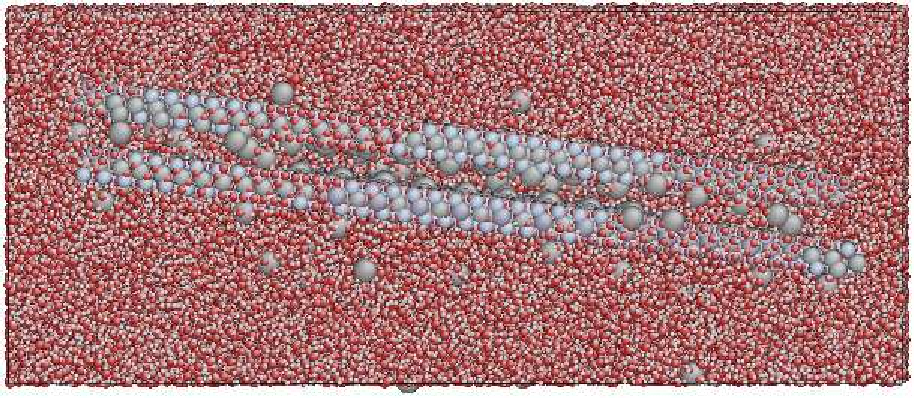
\includegraphics[scale=0.6]{subproject1-bioclays/ymod}
%        \end{center}
%\caption{Visualization of the ingress of water into an isolated clay platelet; the viewpoint is a slice through the clay sheet. Light grey and light blue atoms are the silicon and aluminium atoms of the clay sheet respectively. Oxygen atoms are coloured red and hydrogen atoms are coloured white. Sodium ions, located in the clay interlayer, are dark grey. We can see some sodium ions move away from the surface as the water diffuses through the clay interlayer. }
%\label{Fig:water}
%\end{figure}
% Our previous studies, with periodic boundaries on the clay sheets themselves, were 2/3
%orders of magnitude larger than any previous atomistic simulations of
%clay minerals. They revealed the clay sheets to have some degree of
%flexibility, manifesting as long range, low amplitude undulations with
%wavelengths greater than 25 nm, which are only revealed through
%large scale simulations \cite{jls_2006,thyveetil2007}.  %As an extension 
%to the previous study, we will explicitly include the edges of the 
%clay sheets and the platelet will be completely surrounded by the 
%polymer matrix. The clay platelet will
%consist of  two sheets of $Na^{+}$ montmorillonte clay, which will be
%aligned and staggered relative to each other in two different models.  We
%shall compare the structural and dynamical properties of both the polymer
%and clay platelet to conventional molecular dynamics simulations of
%clay-polymer nanocomposites \cite{cmj_12}.

%\item \emph{Code to be used}
%We will use the scalable molecular dynamics code, LAMMPS \cite{LAMMPS, LAMMPS_2005}, to perform these
%simulations. We will use the rRESPA multi-timestep method \cite{rRESPA} combined with the efficient particle-particle-particle-mesh method \cite{Hockney_book} to calculate the electrostatics. 


%\item \emph{Benchmark Data}
%We have performed comprehensive benchmarks of 
%a hydrated montmorillonite system up to 85 million atoms on Ranger and Kraken.
%See Figure V of the attached `Benchmark Document' for scaling data.

%We find approximately linear scaling up to 2048 processors for 10 million atoms, and up to 4096 for 85 million atoms on Ranger; and up to 2048 for 100 million atoms on Kraken.

\emph{Resource requested:} The simulations to be performed and associated computational requirements are listed in Table \ref{t:claytable}. Each simulation listed of the biopolymer interacting with clay edges will run for 20ns; simulations of the bio-clay systems on the basal clay surfaces will be run for 100ns, to ensure correct conformational sampling of the highly flexible biomolecules is achieved.
 
\begin{table}[!h]
\centering

\begin{tabular}[b]
{|>{\scriptsize}c|>{\scriptsize}c|>{\scriptsize}
c|>{\scriptsize}c|>{\scriptsize}c|>{\scriptsize}c|>{\scriptsize}c|}
\hline
\textbf{Sim Description} & \textbf{No. Sims} &
\textbf{No. Cores} & \textbf{Disk} &
\textbf{Code} & \textbf{TG machine} & \textbf{total SUs}\\
\hline 
Clay edge simulations &  10 & 4096 & 2TB & LAMMPS & Ranger & 2,000,000  \\
\hline
NEMD clay edge simulations & 40 & 4096 & 4TB & LAMMPS & Ranger & 1,000,000 \\
\hline
RNA montmorillonite &  15  & 2048 & 1TB & LAMMPS & Kraken & 500,000 \\
\hline
nucleic-acid LDH & 30 & 2048 & 2TB & LAMMPS & Kraken & 750,000 \\ 
\hline
Grand total of SUs required & & & & & & 4,250,000  \\
\hline
\end{tabular} 
\caption{Summary of biopolymer clay simulations and
simulation times for jobs to be run on Ranger (simulations containing clay edges) and Kraken (interlayer bio-clay composites).}
%\caption{Planned simulations of hydrated
%PEG/$Na^+$-montmorillionite on Ranger 
%(simulations containing clay edges) and Kraken (bio-clay composites).}
\label{t:claytable}
\end{table}
%\end{compactenum}
      
